%% ----------------------------------------------------------------
%% Thesis.tex -- MAIN FILE (the one that you compile with LaTeX)
%% ---------------------------------------------------------------- 

% Set up the document
\documentclass[a4paper, 11pt, oneside]{Thesis}  % Use the "Thesis" style, based on the ECS Thesis style by Steve Gunn
\graphicspath{Figures/}  % Location of the graphics files (set up for graphics to be in PDF format)

% Include any extra LaTeX packages required
\usepackage[square, numbers, comma, sort&compress]{natbib}  % Use the "Natbib" style for the references in the Bibliography
\usepackage{verbatim}  % Needed for the "comment" environment to make LaTeX comments
\usepackage{vector}  % Allows "\bvec{}" and "\buvec{}" for "blackboard" style bold vectors in maths
\hypersetup{urlcolor=blue, colorlinks=true}  % Colours hyperlinks in blue, but this can be distracting if there are many links.

%% ----------------------------------------------------------------
\begin{document}
\frontmatter      % Begin Roman style (i, ii, iii, iv...) page numbering

% Set up the Title Page
\UNIVERSITY {UNIVERSITY OF VERONA}
\department { Department of Computer Science }
\title  {First Year PhD Project Report}
\authors  {\texorpdfstring
            {\href{your web site or email address}{Yonas Teodros Tefera}}
            {Yonas Teodros Tefera}
            }
\addresses  {\groupname\\\deptname\\\univname}  % Do not change this here, instead these must be set in the "Thesis.cls" file, please look through it instead
\date       {\today}
\subject    {}
\keywords   {}

\maketitle
%% ----------------------------------------------------------------

\setstretch{1.3}  % It is better to have smaller font and larger line spacing than the other way round

% Define the page headers using the FancyHdr package and set up for one-sided printing
\fancyhead{}  % Clears all page headers and footers
\rhead{\thepage}  % Sets the right side header to show the page number
\lhead{}  % Clears the left side page header

\pagestyle{fancy}  % Finally, use the "fancy" page style to implement the FancyHdr headers

%% ----------------------------------------------------------------

\pagestyle{fancy}  %The page style headers have been "empty" all this time, now use the "fancy" headers as defined before to bring them back


%% ----------------------------------------------------------------
\lhead{\emph{Contents}}  % Set the left side page header to "Contents"
\tableofcontents  % Write out the Table of Contents

%% ----------------------------------------------------------------
\lhead{\emph{List of Figures}}  % Set the left side page header to "List if Figures"
\listoffigures  % Write out the List of Figures

%% ----------------------------------------------------------------
\lhead{\emph{List of Tables}}  % Set the left side page header to "List of Tables"
\listoftables  % Write out the List of Tables

%% ----------------------------------------------------------------
% End of the pre-able, contents and lists of things
% Begin the Dedication page

\setstretch{1.3}  % Return the line spacing back to 1.3

% Include the chapters of the thesis, as separate files
% Just uncomment the lines as you write the chapters

\chapter{Part One}
\section{Introduction}
This report presents a summary of the doctoral research conducted during my first year of the Ph.D. study, including the plans concerning its progress in the future. The research focuses on studying different methods and challenges in remote teleportation interface design.

In remote robotic teleoperation, with the operator manipulating robotic systems from a distance, the quality of perception of the remote environment plays a central role in the accurate estimation of distances, sizes, movements, and spatial orientations to execute tasks successfully and efficiently. With the advancements in VR and AR technologies, immersive user interfaces could improve human supervisory control of a teleoperation system by providing visual & sensory feedback and remote environment information in an intuitive and easy-to-understand manner.

Most of the traditional interfaces focused on providing video feed-backs in monocular and a stereoscopic 360 videos. which only allow operators to look in a fixed direction. Therefore, in my study, I focused on Interfaces which can give freedom of motion in six-degrees-of-freedom (‘6-DoF’), so that operators see the correct views of an environment regardless of where he is (3 DoF) and where he is looking (+3 DoF).

I conducted my study based on the following research questions: (i) What are the common difficulties of remote teleoperators when they use monocular and stereo video interfaces? (ii) Can we solve these difficulties by providing a 3D reconstruction of the remote environment? (iii) if they can improve, How can we provide the reconstructed environment in real-time with high quality?


\section{Objective}

The main objective of the first part of this Ph.D. research was to investigate how 3D immersive interfaces can be developed to improve interactions in remote teleoperation, and to understand the common effects of this interfaces to the operators?

The study centers on how to design interfaces for risk prevention, task and motion planning without affecting operators mental workload. a more detail description of these points is listed below. 

\textbf{Risk prevention}

Sensors can detect risky situations for humans such as obstacles, collisions, dangerous areas (fire, gas, etc.), and safe / unsafe terrains. Well-designed interfaces can provide timely sensor feedback and allow humans to perceive the risk before it occurs to be able to avoid it.

%To indicate how the terrain is in front of a navigating robot (safe/ unsafe trains).
%To detect and prevent from a collision.
%To find out dangerous areas (fire, gas, etc.) and alert the operator.\\

\textbf{Task and motion planning}

Task and motion planning requires an operator to perceive the environment, decide how to navigate a region, manipulate objects, etc., before the actual task is performed. The operator requires information on the robot kinematics and capabilities in the remote environment. Interactive interfaces can provide information to the operator in the planning phase, with respect to the possible approaches for executing the tasks.

For instance, the following three tasks can be supported by assistive information for the operator.
\begin{itemize}
    \item To find a trade-off for look-ahead possibilities.
    \item To plan the best navigation/optimal trajectory.
    \item To find the best optimal grasping/manipulation points.
\end{itemize}

\textbf{Human factors}

The learning capabilities and the performance of a human operator is limited by the amount of information they can remember and process \cite{NAP25118}. Limitations such as perception, cognition, and physical ergonomics can be supported by designing immersive interfaces \cite{Bowman:2004:UIT:993837}.\\
To support and guide this study, the following questions are considered, among others.
\begin{itemize}
    \item How to present information without confusion?
    \item How to find a balance in showing information and for how long to show it?
    \item How to represent the multi-dimensional information (environmental sensors, point-clouds, camera streams, etc.) effectively and efficiently?
    \item How operators perceive different information?
    \item What are the perceptual and cognitive constraints in remote teleoperation?
    \item How to integrate different sensory information in an ergonomic and user-friendly manner, while utilizing human cognitive capabilities?
\end{itemize} 

\section{State of the Art}

%\section {Factors That Affect Remote Teleoperation}
%the General procedures should be what progress in those two months ?
%why this specific literature review needed?
%What I understood ?
%How can we use it ? 
%What limitations are there ?

To reach a comprehensive understanding of the research area, I have been doing a general literature review beginning with the research questions listed below. Figure \ref{Reviewed Papers} shows the total number of papers (155) reviewed. they are selected from database and publisher websites.

I started my literature review by reviewing papers about 3D user interfaces and related Human factors. These papers cover 16 $\%$ of the total study. Following the first study, I continued my literature review on  Augmented Reality interfaces for remote teleoperation. this study covers 74 $\%$ of the total papers reviewed.  based on these studies, the remaining 9.1 $\%$ of the total study focused on real-time 3D reconstruction for a dynamic environment.

\begin{itemize}
    \item What are the common problems of remote teleoperators when they use monocular and stereo video interfaces?
    \item What is the effect of Augmented Reality Interfaces for remote teleoperation?
    \item How operators interact with field robot with virtually replicated 3d environments?
\end{itemize}

\begin{figure}
     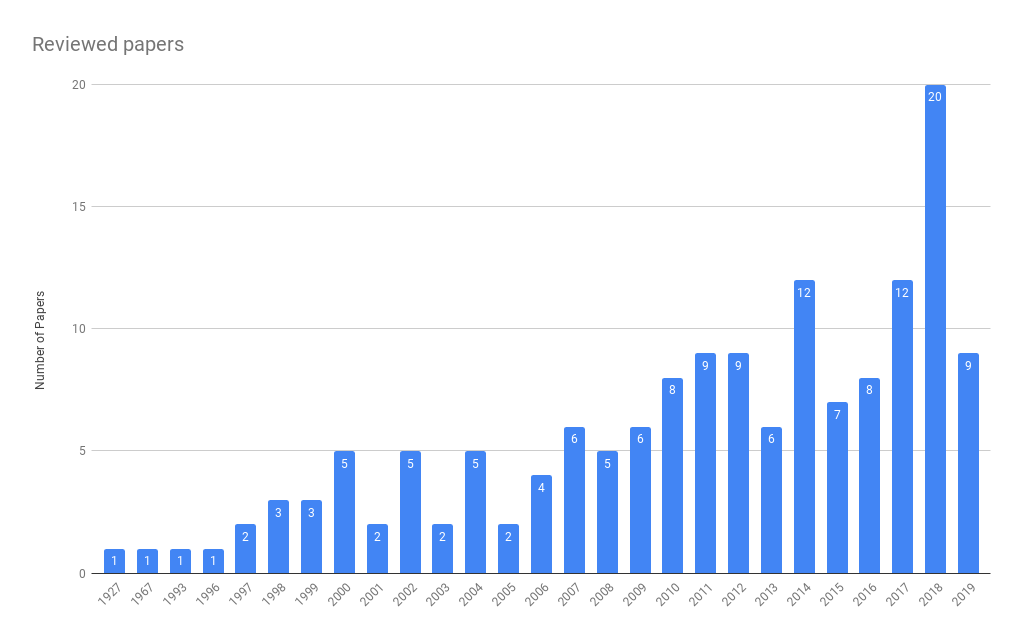
\includegraphics[scale=0.35]{images/Reviewed_papers.png}
    \caption{Reviewed Papers}
    \centering
    \label{Reviewed Papers}
\end{figure}

\subsection{Factors, which affect remote teleportation}

This part of the literature review discuss on how the human operator process information and what are the different factors that affect remote teleportation: especially related to a field of view (FOV), limited depth perception, network latency and as such.

\underline{Human factors:} Bowman et.al  \cite{Bowman:2004:UIT:993837} refers the term human factors as the capabilities; characteristics; limitations of the human user; and includes considerations related to the body (acting), the sense(perceiving), and the brain(thinking).

A Basic knowledge of how operators process information into useful (inter)action is very valuable to understand the human factors and it is called information processing \cite{Bowman:2004:UIT:993837}. Information processing has been studied for many years and different studies have designed different models. Bowman et al. \cite{Bowman:2004:UIT:993837} adapted a high level staged information processing model from \cite{PMID:11540969} by mapping it into the three main factors: perception, cognition, and physical ergonomics figure \ref{Info Processing}.

According to Bowman et al. \cite{Bowman:2004:UIT:993837} model, a stimuli or events which are perceived will be provided with a meaningful interpretation based on memories of past experiences. In response to what is perceived, actions may get selected, executed or information may get stored in working memory,(short-term memory).

\begin{figure}
     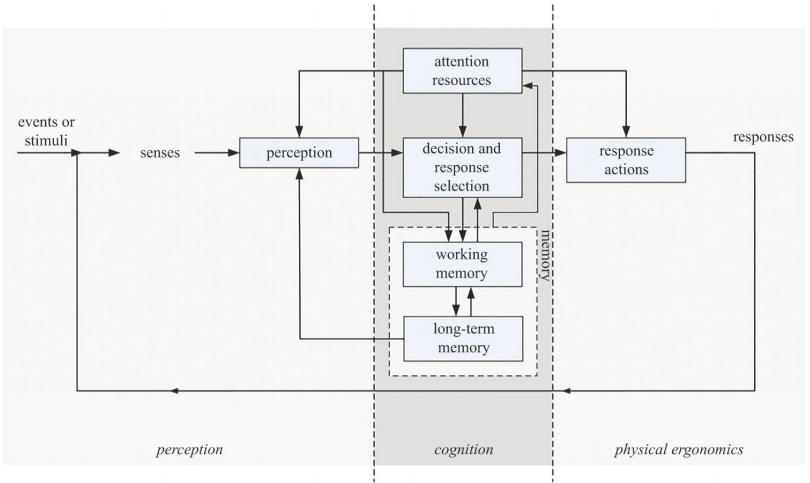
\includegraphics[width=1\textwidth]{images/Info_proc.png}
    \caption{Information processing and related human factors adapted from \cite{PMID:11540969}.}
    \centering
    \label{Info Processing}
\end{figure}


\underline { Attention Resources :} Attention can be seen as a selection process and it could be used to draw attention to specific information from the dynamic spatio-temporal environment.

Attention process is prone to errors, which can be raised by certain bottlenecks, which leads to an inability to notice visual (change blindness) and audition changes ( ‘change blindness’ refers to the surprising difficulty observers have in noticing large changes to visual scenes \cite{SIMONS200516}). Similarly, errors occur on a temporal basis, especially when rapid sequences of stimuli occur.

\underline {Short and long term memories:} 
Working memory has a limited capacity and attention resources highly influence it. in contrast, the capacity of our long-term memory is vast; storing information about our world, concepts, and procedures while not being directly affected by attention \cite{Bowman:2004:UIT:993837}.

In addition to different factors related to human factors, I studied different technological factors. which can affect remote teleoperation and the operators. 

\underline {Field of View :} 
Cameras with limited angular view create the so-called "Keyhole" effect (a sense of trying to understand the environment with its narrow "Soda Straw" field of view). major consequences of this effect include missing new events, increased difficulty in navigating novel environments, gaps or incoherent models of the explored space \cite{woods2004envisioning}.

\underline {Orientation and Attitude of the robot:} 
When the remote environments become more complex and cues to a robot’s pose become sparser: it becomes easy for a teleoperator using an egocentric (camera) display to lose situational awareness. To successfully navigate locally and Globally to know where the object of interest is, The operator needs to know the robot's attitude (i.e., pitch and roll) to avoid roll-over accidents \cite{wang2004gravity}.

\underline{Orientation in the Remote Environment:} Navigation with a traditional (north-up) map can be challenging at times because of the demand of mental rotation. track-up (ego-referenced; rotating viewpoints) maps consistently show that track-up maps are better for local guidance (i.e., navigation) and north-up maps are better for global awareness \cite{wang2004gravity}.

\underline{Attitude of the robot:} Attitude (i.e., pitch and roll) of a robotic vehicle may be easy to reference when there are other familiar objects (e.g., horizon, buildings, trees, etc.) in the remote environment. However, if those reference points are absent and the onboard cameras are fixed, operators sometimes find it surprisingly hard to accurately assess the attitude of their robotic vehicles \cite{wang2004gravity}.

\underline{Multiple camera and View point:}
The capabilities to see the robot and its local environment gives the operator a better sense of the robot’s location with respect to obstacles, victims, or other potential difficulties \cite{keyes2006camera}. However, the difference in eye point and camera viewpoint could create motion sickness.In addition, when handling multiple robots, it can be challenging for the operator to acquire different contexts rapidly when switching among robots: information in one scene may not be encoded sufficiently to be compared/integrated when accessed subsequently ( change blindness).

\underline{Degraded Depth Perception :}
Degraded depth perception affects the teleoperator’s estimates of distance and size and can have profound effects on mission effectiveness. In the case of monocular cameras, the operators have to rely on other cues: such as shadows, linear perspective and size consistency.

The effect of degraded depth perception has a higher impact when working in unfamiliar and difficult terrain due to lack of apparent size. In addition, remote manipulation that involves ballistic movement, recognition of unfamiliar scenes, analysis of three-dimensionally complex scenes and the accurate placement of manipulators or tools within such scenes \cite{drascic1993investigation}.

\underline{Degraded Video Image and Time delay :}
Degraded video feeds could leave out essential visual cues for building teleoperators mental models of the remote environment. Different factors such as low bandwidth, low frame rate, low resolution and the number of bits per pixel can create degraded video feeds.

\underline{Motion :}
Teleoperation can be difficult and distracting because of the moving platform vibration.which makes viewing the visual displays and manual control/input more challenging \cite{schipani1998quantification}.

\begin{longtable}{p{2.5cm} p{5cm} p{5cm} p{1cm}}
    \hline
      \textbf{Factor} & \textbf{Effects} & \textbf{Suggested solution} & \textbf{Ref.\#}\\
            \hline
            \rowcolor{lightgray} 
           Short and long term memories &
           \begin{enumerate}[noitemsep,nolistsep]
                \item Working memory has a limited capacity.
                \item Long term memory has a slower recall. 
           \end{enumerate} &
           \begin{enumerate}[noitemsep,nolistsep]
           \item Minimize the need for a mighty memory.
           \item Present information in an organized way.
           \item Place all information in close physical proximity.
           \item give the operator control over the information.
           \end{enumerate}
             & 
            \cite{Bowman:2004:UIT:993837}\\
        \hline
          
                Attention resources &
                \begin{enumerate}[noitemsep,nolistsep]
                    \item Working memory is highly affected by attention resources.
                    \item Is prone to errors, which can lead to an inability to notice visual and audition changes.
                \end{enumerate} &
                \begin{enumerate}[noitemsep,nolistsep]
                \item Don't litter the side of the interface with destructible materials.
                \item Focus the operators’ attention on important elements.
                \end{enumerate} &
                \cite{SIMONS200516} \cite{Bowman:2004:UIT:993837} \cite{PMID:11540969}\\
                
                \hline
     \rowcolor{lightgray}
       Decision-Making &
           \begin{enumerate}[noitemsep,nolistsep]
           \item The speed of decision-making processes varies widely, and is affected by conflicts, complexity, or uncertainty of either the information being processed or the detection of the possible outcome.
           
           \end{enumerate} &
            \begin{enumerate}[noitemsep,nolistsep]
            \item Behaviour can be adjusted by emotional state and conditioning.
            \item  Skills allow users to make more accurate and quicker responses.
            \end{enumerate} &  \cite{pavlov1927conditional} \cite{Bowman:2004:UIT:993837} \cite{fitts1967human} \\
            
    \caption{Summery of Human related factors.}
    \label{table:human factors}
    \end{longtable}

 \begin{longtable}{p{2.5cm} p{5cm} p{5cm} p{1cm}}
    \hline
      \textbf{Factor} & \textbf{Effects} & \textbf{Suggested solution} & \textbf{Ref.\#}\\           
            
        \hline 
        Field of View  &
           \begin{enumerate}[noitemsep,nolistsep]
           \item Restricted FOV affects  target detection and identification.
           \item Distance cues may be lost and depth perception may be degraded.
           \item Degraded remote driving.
           \item Increased difficulty in navigating novel environments.
           \end{enumerate} &
            \begin{enumerate}[noitemsep,nolistsep]
            \item Wider FOV (changeable FOV ) can be used. 
            \item Stereoscopic 3D displays.
            \item Multiple cameras and single cameras with special optics.
            \end{enumerate} &  \cite{Chen2014} \cite{smyth2000indirect} \cite{van2003image} \cite{Chen2007HumanPI} \cite{Suzuki2014} \\
        \hline
          
     \rowcolor{lightgray} Orientation and Attitude of the Robot &
           \begin{enumerate}[noitemsep,nolistsep]
           \item Difficulty knowing the robot orientation in the environment.
           \item North up and tracked-up map.
           \item Mismatch between actual and perceived attitude of robot.
           \item Unawareness of robot's inclination and shape.
           \end{enumerate} &
            \begin{enumerate}[noitemsep,nolistsep]
            \item Track-up map for navigation.
            \item North-up map for tasks involving integration of spatial relations in the environment.
            \item Gravity referenced view.
            \end{enumerate} &  \cite{wang2004gravity} \cite{Chen2007HumanPI} \cite{fitts1967human} \cite{drury2006changing}\\
        \hline
         Multiple camera  and View point &
           \begin{enumerate}[noitemsep,nolistsep]
           \item Attention switching and change blindness.
           \item Motion sickness.
           \item Egocentric: cognitive tunneling.
           \item Exocentric: loss of immediacy and true ground view.
           
           \end{enumerate} &
            \begin{enumerate}[noitemsep,nolistsep]
            \item Auditory alerts.
            \item Multi-modal solutions.
            \item Peripheral cues for egocentric.
            \end{enumerate} &  \cite{keyes2006camera} \cite{Chen2007HumanPI} \cite{olmos2000tactical} \cite{keyes2006camera} \cite{Chen2007HumanPI} \cite{olmos2000tactical}\\
        \hline

        \rowcolor{lightgray} Depth perception &
           \begin{enumerate}[noitemsep,nolistsep]
           \item Underestimation of distance and size.
           \item Degraded navigation, driving, and telemanipulation.
           \end{enumerate} &
            \begin{enumerate}[noitemsep,nolistsep]
            \item Sterioscopic displayes (SDs).
            \item Inter-camera distance should be less than inter-ocular distance.
            \end{enumerate} &  \cite{Bowman:2004:UIT:993837} \cite{fitts1967human} \cite{Chen2007HumanPI}\\
        \hline 
        
        Video frame rate and Time delay.
         &
           \begin{enumerate}[noitemsep,nolistsep]
           \item Degraded motion perception and spatial orientation.
           \item Degraded target identification and latency.
           \item Motion sickness.
           \item Over actuation when delay is variable.
           \end{enumerate} &
            \begin{enumerate}[noitemsep,nolistsep]
           \item Utilize the human cognitive processing speed which is around 170 ms (range: $75-370$ ms).
            \item Augmented reality/ overlaying information.
            \item Predictive Display (simulation in VR/AR).
            \item Robust adaptive algorithm.
            \end{enumerate} &  \cite{madl2011timing} \cite{Chen2007HumanPI} \cite{kebria2019robust} \\
      
        \hline
      \rowcolor{lightgray} Motion &
           \begin{enumerate}[noitemsep,nolistsep]
           \item Degradation on accuracy and latency.
           \item Motion sickness.
           \end{enumerate} &
            \begin{enumerate}[noitemsep,nolistsep]
            \item Multi modal user interface.
            \item Tailor interface to vibratory and motion effects.
            \end{enumerate} &  \cite{kamsickas2003future} \cite{schipani1998quantification}\\
        \hline

\caption{Summery of different technological factors.}
\label{table:tasks}
\end{longtable}

\subsection{Augmented Reality Interface for Teleoperation}
This part of the literature review explains how I used a systematic literature review to select research works related to Augmented reality interfaces for remote teleoperation. To add a depth and guide to the study, I defined the following four research questions.

\begin{itemize}
    \item How situational awareness is achieved in teleoperation using AR interfaces ?
    \item What are the different challenges of Augmented Reality in Teleoperation ?
    \item What are the range of applications of AR in Teleoperation ?
    \item what are the most suitable immersive interfaces for teleoperation ?
\end{itemize}

Papers were identified by means of a structured keyword search from the following major databases and publisher websites.

\begin{itemize}
    \item IEEE Xplore (http://ieeexplore.ieee.org/)
    \item Scopus (www.scopus.com).
    \item ScienceDirect (https://www.sciencedirect.com/)
    \item ACM (https://dl.acm.org)
\end{itemize}\\

Keywords such as \textbf{Teleoperation; telepresence; Augmented Reality;Mixed Reality; teleoperator ; telerobotics} were combined as such.
\begin{itemize}
    \item ("Teleoperation " AND ("Augmented Reality" OR "Mixed Reality")).
    \item ("Teleoperation" OR "Teleoperator") AND ("Augmented Reality" OR "Mixed Reality").
    \item ("Teleoperation" OR "Telerobotics") AND ("Augmented Reality" OR "Mixed Reality").
\end{itemize}

However, In order to align the research papers with the research aims inclusion and exclusion criteria  defined by language(only articles in English) and restriction by primary articles (excluding secondary studies such as other systematic reviews, area mapping and surveys).

The over all sample papers considered in this study were 508 (IEEE=96, ACM=101, Scopus=211, Sciencedirect=100): before applying the exclusion criteria) and 139 research papers after applying the exclusion criteria.

\begin{figure}[h]
    \centering
    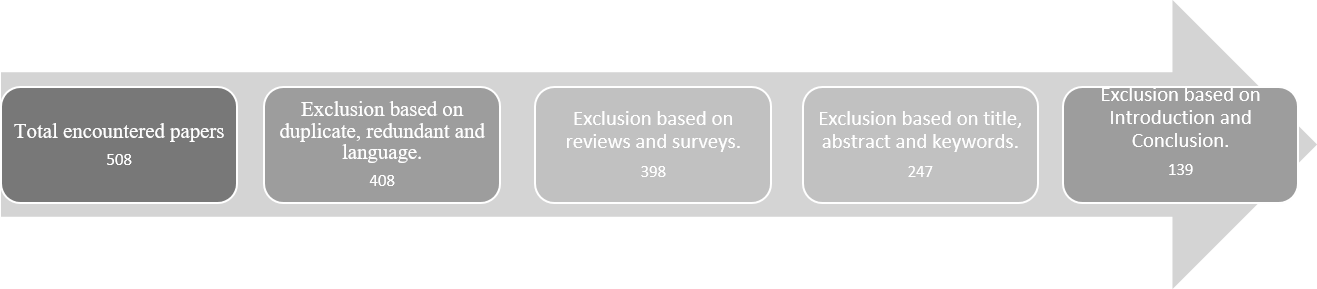
\includegraphics[width=0.8\textwidth]{images/Selected_papers.png}
    \caption{Number of Selected papers}
    \label{fig:PapersNumber}
\end{figure}

To characterise the papers, a bibliometric analysis of these initial 508 research papers and the final set 139 research papers was performed by using VOSviewer software and it reveals the most frequent keywords. To obtain more information about these keywords, a colour-coded graph of their density was produced \ref{fig:final Density}. The colour distribution is between blue and red. The greater the number of items near a point and the greater the weight of neighbouring items, the closer the keyword is to red. On the contrary, the smaller the number of items in the neighbourhood of a point and the smaller the weights of neighbouring items, the closer the keyword is to blue.keywords such as 'Augmented Reality','Teleoperation','Telerobotics','Navigation','Mixed Reality' and 'Telepresence' appeared with the greatest density.

\begin{figure}[h]
    \centering
    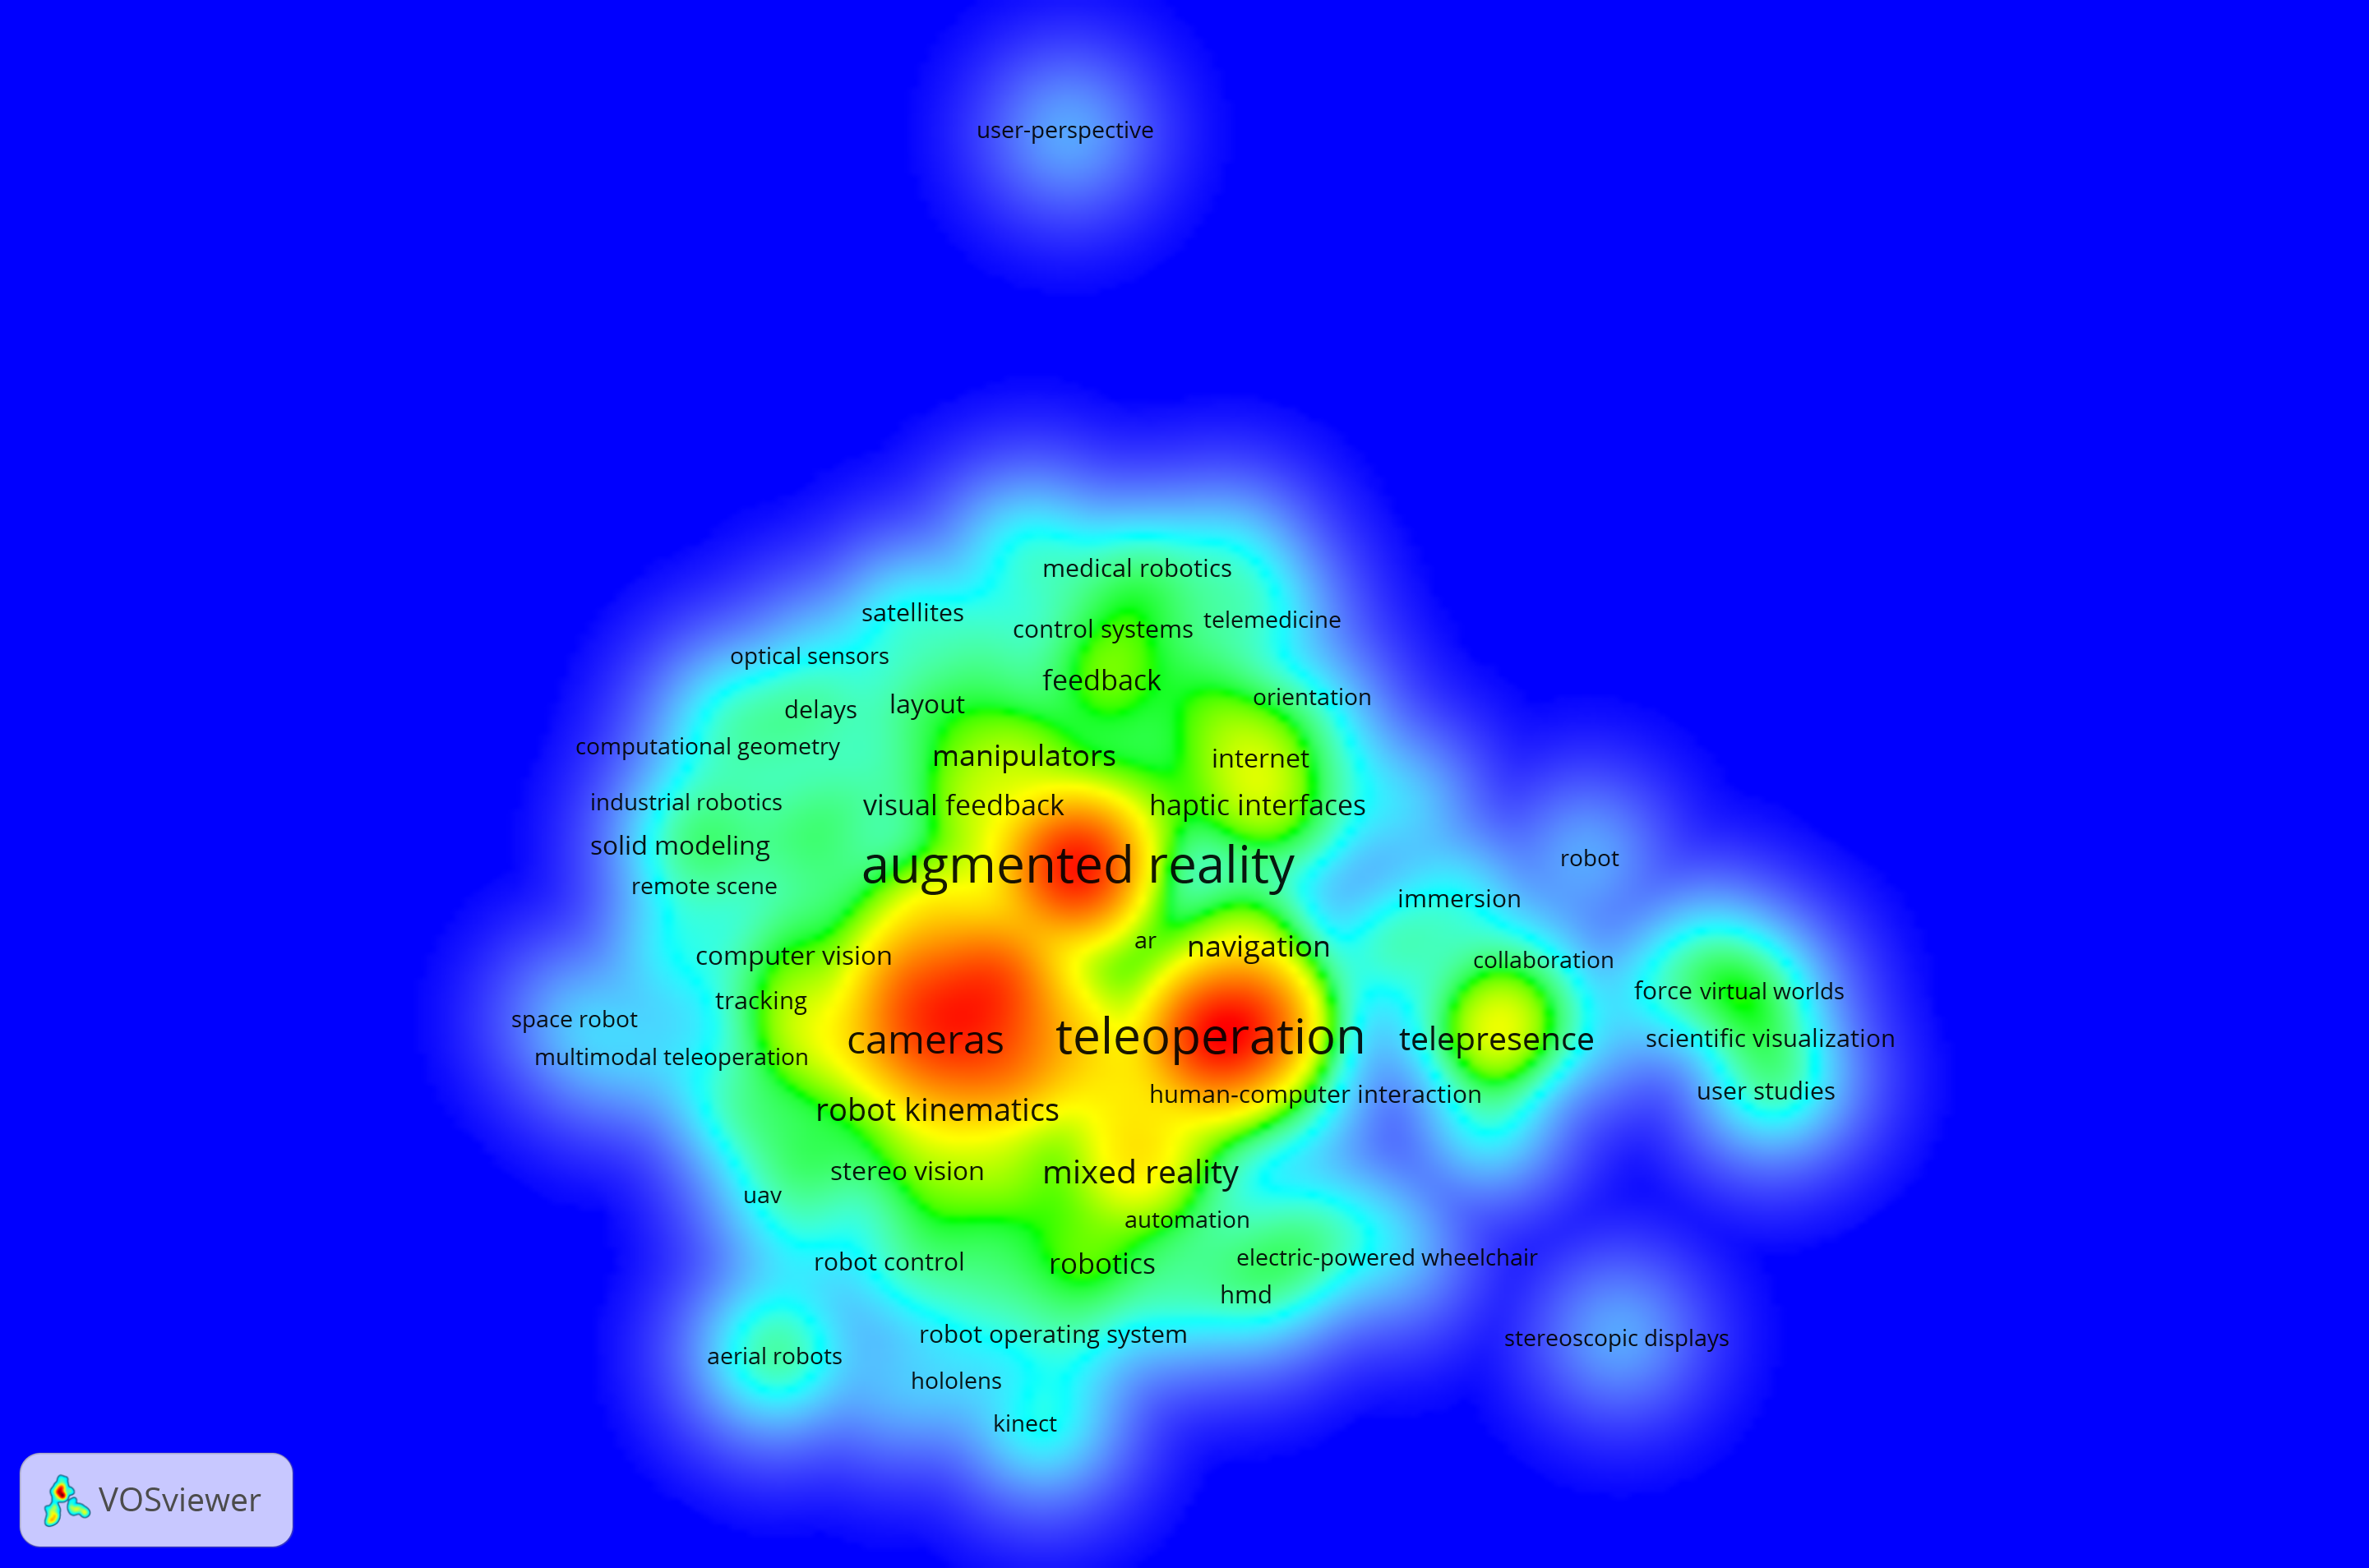
\includegraphics[width=0.7\textwidth]{images/Density_3.png}
    \caption{Mapping of the most frequent keywords of the final set of research papers}
    \label{fig:final Density}
\end{figure}

To investigate the range of applications of AR in Teleoperation the final set of the papers were verified. Figure \ref{fig:range of applications} shows the 4 broad categories that appear most.
 
To define the  major categories, I adapted the procedure used in \cite{7912316} and I categorized them into navigation, manipulation, simulation, and virtualization categories.
 
The first category was Navigation, which includes papers used for Localization, geonavigation, geovisualizations of interactive maps, landscape visualizations, to indicate safe navigation and for free view points indication. This are around 43 papers, about 37.4 $\%$ of the papers in the set.
 
The second category was manipulation, application such as overlaying information, information about the target and instructions for task execution are categorized together. This were around 48 papers, about 41.7 $\%$ of the papers in the set.
 
Papers which use AR for Flight and drive simulation using surrogates, for collision detection before deployment and task planning are categorised in the group Simulation.This are around 15 paper , about 13 $\%$ of the papers in the set.
 
The remaining 9 papers, about 7.8$\%$. used for conference and training application are classified as a Virtualization group.
 
\begin{figure}[h]
    \centering
    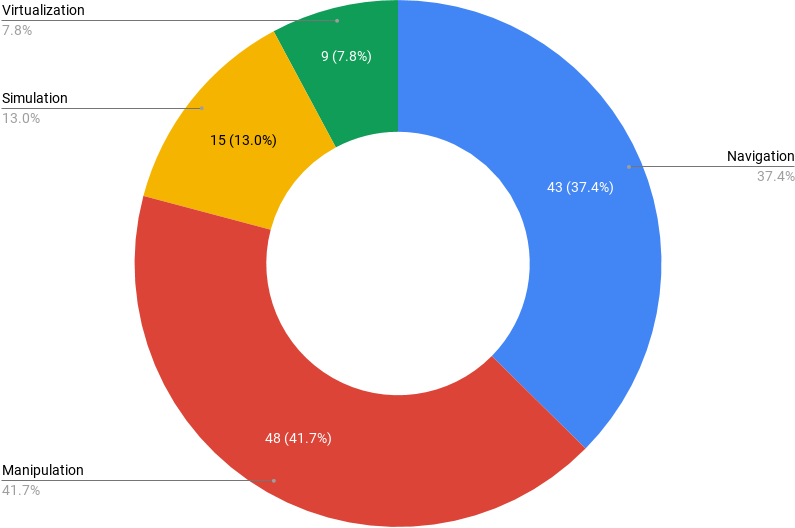
\includegraphics[width=0.5\textwidth]{images/chart.png}
    \caption{Range of applications where AR is used in teleoperation.}
    \label{fig:range of applications}
\end{figure}

\subsection{Real-time 3D Reconstruction for Teleoperation}

This part of the literature review explains how I used In this section I was exploring the representation of remote environment (In 3D point clouds and Mesh) and convincingly reconstruct the visual dynamics of the real world in real-time and provide it in intuitive way. For e.g., showing the 3D reconstruction of the environment to the operator in real-time as the remote robot moves through the field.

\textbf{3D Reconstruction}


3D reconstruction of static environments has its roots in several areas within computer vision and graphics.Although there are many different algorithms for RGB-D reconstruction of static scenes, most of these approaches have a very similar processing pipeline \cite{Zollhofer2018}, which I describe here for reference \ref{fig:staticDynrec} Left.

\begin{figure}[h]
    \centering
    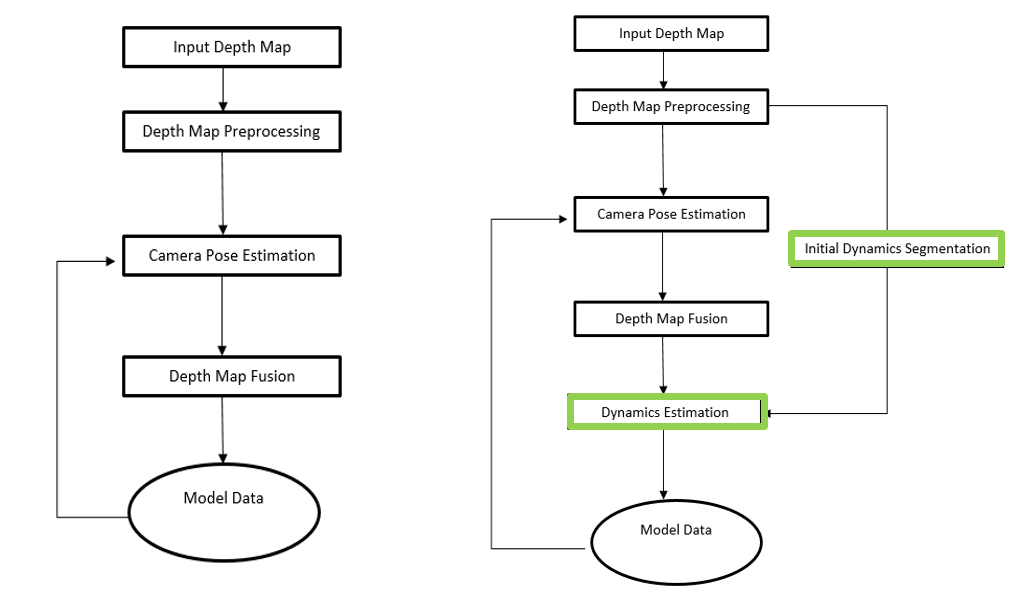
\includegraphics[scale=0.5]{images/Static_Dynamic_reco.PNG}
    \caption{Left: 3D reconstruction for static environment and Right: 3D reconstruction for Dynamic environment pipeline}
    \label{fig:staticDynrec}
\end{figure}

\begin{figure}[h]
    \centering
    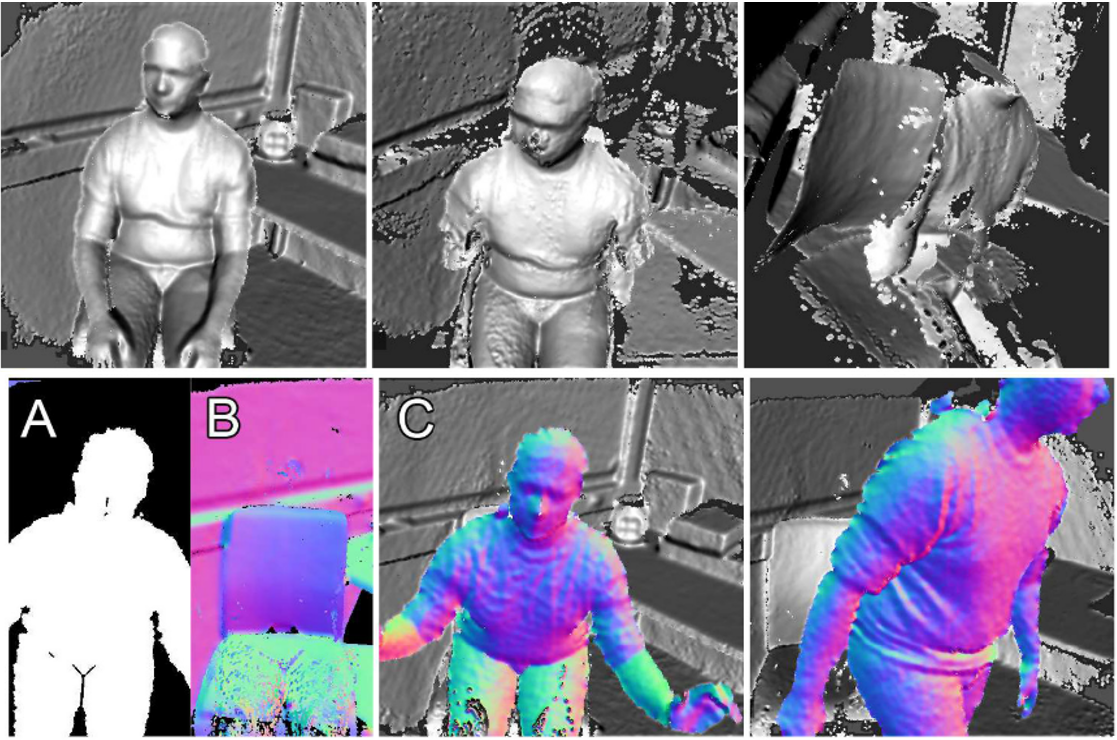
\includegraphics[scale=0.5]{images/static_and_dynamic_failure.PNG}
    \caption{Top: Static environment reconstruction failure and Bottom: Dynamic reconstruction \cite{Keller:2013:RRD:2544744.2544784}.}
    \label{fig:staticfailure}
\end{figure}

In the first stage, the Depth Map Preprocessing, noise reduction and outlier removal is applied to the incoming RGB-D data. Depending on the following stages, additional information is derived from the input range map and stored in additional input maps. In the subsequent stage, the Camera Pose Estimation, the best aligning transformation for the current frame is computed. This can be achieved in a frame-to- frame, frame-to-model, or global fashion. Finally, all points from the current input frame are transformed with the estimated transformation and are merged into the common model in the Depth Map Fusion stage \cite{Zollhofer2018}.

3D Reconstruction for static environments \textbf{assumes the environment is static and moving objects detected as an outlier and ignored}. in addition this it can create a failure of camera tracking see figure \ref{fig:staticfailure} Top. This could create a Miss- perception of the scene and can create a confusion to the operator.

\textbf{Dynamic 3D Reconstruction}

In addition to static components, many natural environments contain dynamic objects. for such reasons a real-time-dynamic environment reconstruction system is needed. More recently, many people have begun to work on this area. The approach works by classifying the dynamic scene into static and dynamic parts.then, the camera motion and the dynamic parts of the scene are segmented and reconstructed separately figure\ref{fig:staticfailure} bottom.The approach \cite{Keller:2013:RRD:2544744.2544784} computes a foreground segmentation based on scene dynamics (A) and excludes them from camera pose estimation (B). This enables robust camera tracking even if large parts of the scene is moving (bottom). 

More recently, many people have begun to leverage Deep Neural Networks and their ability to learn from large amounts of training data to improve Dynamic 3D reconstruction.They categorised this approaches into three main directions.One deforms the whole world in a non-rigid manner in order to include a moving object \cite{newcombe2015dynamicfusion}.The second specifically aims at building a single static background model while ignoring all possibly moving objects and thus improving the accuracy of camera tracking \cite{jaimez2017fast} \cite{scona2018staticfusion} \cite{barnes2018driven}\cite{bescos2018dynaslam}.The third models dynamic components by creating sub-maps for every possibly rigidly moving object in the scene while fusing corresponding information into these sub-maps \cite{runz2017co} \cite{barsan2018robust}\cite{runz2018maskfusion} \cite{xu2019mid} \cite{narita2019panopticfusion} \cite{ miksik2019live} \cite{strecke2019fusion} \cite{hachiuma2019detectfusion}.

The reconstruction of dynamic scenes is \textbf{computationally and algorithmically more challenging } than its static reconstruction counterpart. Modeling the non-rigid motion of general deforming scenes requires orders of magnitude more parameters than the static reconstruction problem. In general, finding the optimal deformation is a high-dimensional and highly non-convex optimization problem that is challenging to solve, especially if \textbf{real-time performance} is the target (state of the art dynamic 3D reconstruction works at a maximum of 5Hz \cite{inproceedings}).

\section{Report on progress}

Remote  teleoperation  relies  on  communication  networks,  with  limited  bandwidth,  low  frame  rates,  low  resolution,  etc.  These  aspects  result  in  degraded  video  feeds  and  point-clouds,  which  can  leave  out essential visual cues for the operator’s mental models of the remote environment. As noted above, in VR-based teleoperation, the operators rely heavily on the visual cues to understand their location, and their relative range with respect to the task space. 
As part of my initial study , I have been designing and experimenting different methods of low latency video streaming , marker based Augmented Reality interface design , implementing 3d Reconstruction for static environment and Point Cloud Streaming from multiple depth sensors.

\textbf{Augmented Reality Interface}

One way to restore the visual cues is to enhance the VR scene itself by overlaying the objects from the real-world environment with the corresponding virtual 3D meshes in the VR scene. The AR interface, as  described  in  [1],  can  help  the  operator  overcome  the  difficulties  of  perception  by  guiding  the  operator using virtual overlays in their view.

Marker-based AR algorithms can be used to overlay 3D Meshes or informations on top of a  pre-defined “marker” patterns. Figure 19 shows the concept with the real-world scene, the virtual scene,  and  the  3D  meshes  overlaid.  The  example  task  shown  here  is  the  peg  attached  as  the  end-effector of the UR5, to be inserted in the hole located on the wall. The 3D meshes of the peg and the hole are seen in the 

\begin{figure}[h]
    \centering
    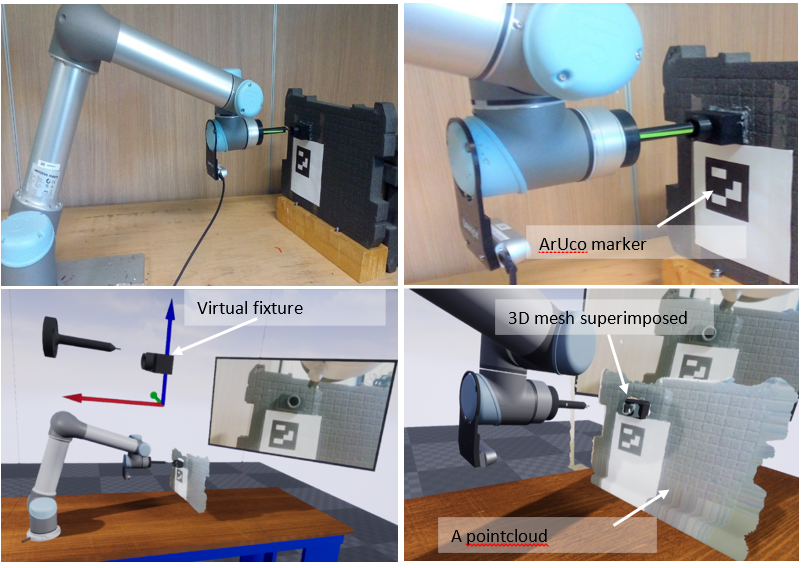
\includegraphics[scale=0.5]{images/Aruco_AR.PNG}
    \caption{Augmented Reality  interface  for  scene enhancement of the remote environment and virtual fixture based guided teleoperation.}
    \label{fig:Aruco_AR}
\end{figure}\\

Associating the real-world objects with the 3D meshes is possible by attaching markers to the objects of  interest  in  the  physical  world  and  by  extracting  their  identifier  in  the virtual  world.  A  popular  approach  for  this  is  to  use  square  fiducial  markers  (ArUco  markers),  shown  in  Fig. \ref{fig:Aruco_AR} top right  image.  This  marker is a synthetic square marker composed of a wide black border and an inner binary matrix that forms its identifier. Custom code has been developed that provides acquisition of videos from the cameras as well as camera pose tracking using the ArUco markers. The following stages are involved in the process:

\begin{itemize}
    \item Based on known objects in the real-world, 3D meshes of the objects are generated, which can be used as overlays within the VR scene. 
    \item Printed AruCo markers are placed next to the objects in the real-world, in such a way as to be visible in the camera view. Each object gets a unique identifier for the marker.
    \item The  relative  position,  orientation,  and  the  identifier  of  the  marker  are  calculated  using  the  OpenCV libraries. Based on the extracted identifier, the corresponding 3D mesh is introduced in the virtual scene. 
\end{itemize}


Two different methods have been adopted to assist the operator using the 3D mesh in the VR scene.

\begin{itemize}
    \item \textbf{Point-cloud  enhancement:}  As  seen  in \ref{fig:Aruco_AR},  the  point-cloud  is  visible  to  the  operator  within the VR scene, allowing depth information when interacting with objects. With this AR interface,  the  3D  meshes  can  be  overlaid  directly  over  the  point-cloud at  the  position  and  orientation  of  the  real-world  object.  This  is  seen  in  Fig. \ref{fig:Aruco_AR} bottom right,  where  the  3D  mesh  is  visible  clearly, in addition to point-cloud. This method allows the operator to see the complete object in  VR,  instead  of  just  the  parts  of  it  coming  from  the  point-cloud.  Additionally,  the  mesh  remains in place even if the point-cloud is turned-off.
    
    \item \textbf{Virtual fixture tool:} This is an independent way of visualizing the meshes in the VR scene. It provides a close-up view of the 3D objects of interest, in   this case, the peg and the hole, in a separate space in the VR scene (Fig. \ref{fig:Aruco_AR} bottom left). As a virtual fixture, the tool can be zoomed into or out,  rotated,  and/or  scaled  to  allow  better  understanding  of  the  target  task  and  closer  visualization of the interacting objects. With fluid mapping between the teleoperator and the VR scene, as described above, this eliminates the need of “teleporting”, i.e., moving around in the virtual space.
    
\end{itemize}

In either case, the position and orientation of the 3D meshes in the VR scene need to be updated in real-time based on the calculated translation and rotation of the markers in the camera view.

\textit{Analysis: What are the challenges?}
\begin{itemize}
    \item Markers doesn't exist in real-World.
    \item Pri designed 3D models doesn't represent the actual state of the world.
    \item limited to a certain number of objects.
\end{itemize}


\textbf{Multiple camera and Point-cloud Streaming}

One of the important requirement of remote teleoperation is to have low latency, high-quality video and point cloud streaming between the MASTER and FIELD robot with low bandwidth consumption. To meet this requirement I have designed multiple cameras and point-cloud streaming algorithms on embedded computing board (Jetson Xavier). The Xavier incorporates hardware acceleration (GPU) for encoding various coding standards using its NVIDIA Multi-Standard Video Encoder.

Figure \ref{fig:StreamingPipe} shows A Video and point cloud streaming architecture with detail components pipeline. Point cloud and RGB data, which are acquired from the two Real sense (RS 1 and RS 2) and ZED (ZED 1 and ZED 2) cameras are processed before given to streaming pipeline. Subsequently, a multithreaded algorithm splits it into video and point cloud data and supplies it into the two streaming pipelines simultaneously. 

\begin{figure}[h]
    \centering
    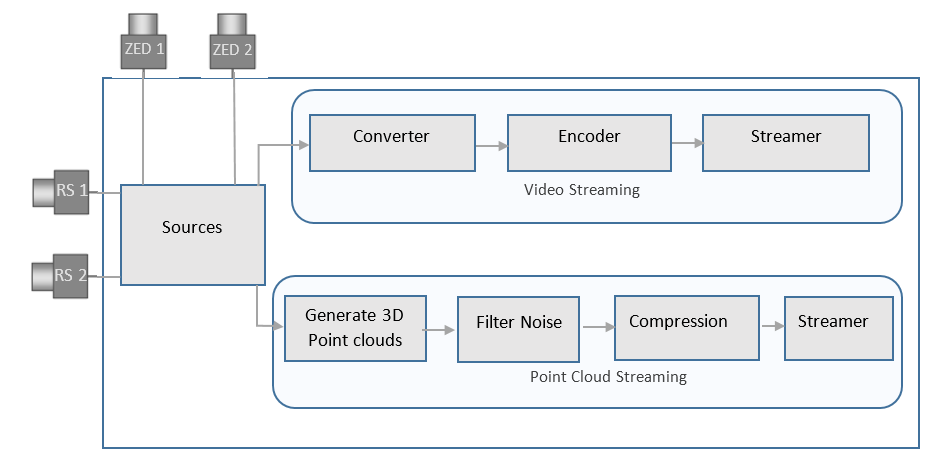
\includegraphics[scale=0.4]{images/Video_Point_Streaming.PNG}
    \caption{A Video and point cloud streaming architecture with detail pipeline.}
    \label{fig:StreamingPipe}
\end{figure}\\


\begin{figure}[h]
    \centering
    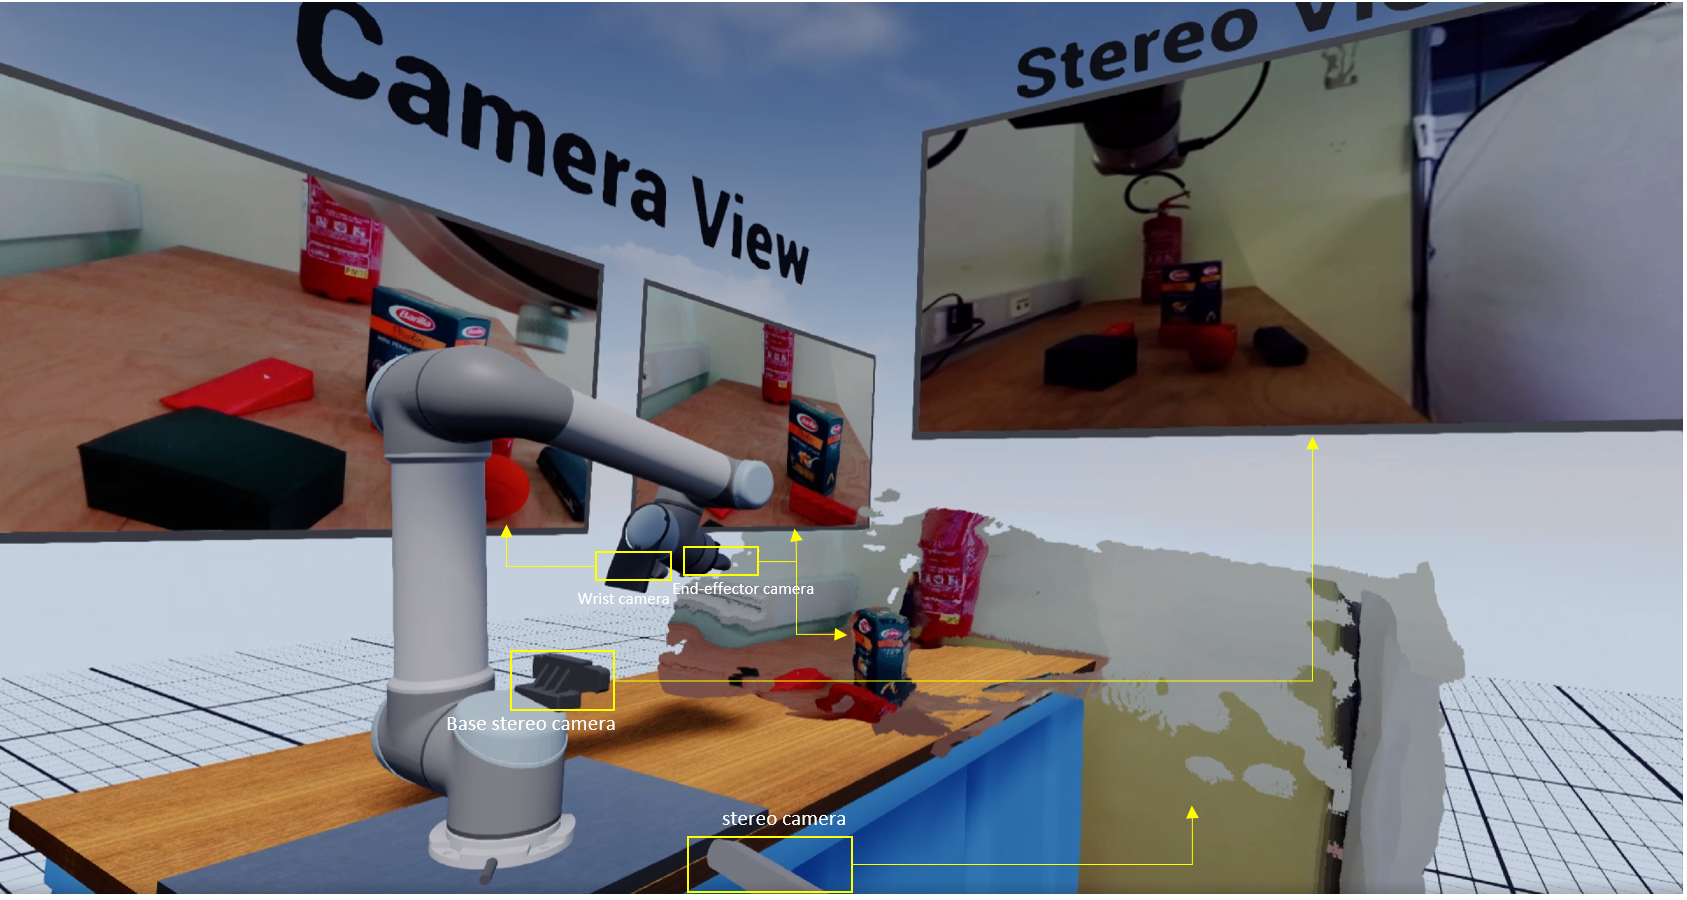
\includegraphics[scale=0.2]{images/Point_cloud_multipl_1.PNG}
    \caption{A Video and point cloud display in virtual reality.}
    \label{fig:StreamingPipe}
\end{figure}\\


The video streaming pipeline uses video transcoding components that involve a three-step process. First, the video file is converted to an uncompressed format. Second, this uncompressed format is then encoded into the target format and finally streamed to the MASTER station. The detail description of each component is listed below:
\begin{itemize}
    \item \textbf{Converter:} This component converts from one color space (e.g. RGB) to another one (e.g. YUV). It can also convert between different YUV formats (e.g. I420, NV12, YUY2 …) or RGB format arrangements (e.g. RGBA, ARGB, BGRA…).
    \item \textbf{Encoder:} This component encodes the raw video coming from the convert element into H264 compressed data, also otherwise known as MPEG-4 AVC (Advanced Video Codec). The element uses a hardware-based encoder (referred to as NVENC) \cite{pgv20181093} , which provides fully accelerated hardware-based video encoding.
    \item \textbf{Streamer:} I have implemented a streaming protocol, which uses Real-time Transport Protocol (RTP) to deliver the video over IP networks to the master station. The Stream element uses a gstreamer udpsink that sends UDP packets to the network.  

\end{itemize}

The point-cloud streaming pipeline acquires 3D data from ZED and real-sense camera. Which consist of huge point sets describing three-dimensional points associated with additional information such as distance, color, normals, etc. with high rate and occupy a significant amount of memory resources and bandwidth. To transmit this data over rate-limited communication channels, methods for filtering noise and compressing are designed.The detail description of each component is listed below: 

\begin{itemize}
    \item \textbf{Generate 3D Point clouds:} This component generates takes 3D depth data from the Realsense and ZED camera and generates 3D point-clouds.
    
    \item \textbf{Filter Noise:} This component filters noise and outliers, which are coming from measurement errors.
    \item \textbf{Compression:} This component exploits the spatial temporal redundancies in point clouds to compress the 3D point cloud. This component uses the PCL Octree based compression codec \cite{kammerl2012real}, which is based on the octree data structure and uses an inter-frame XOR-based codec for temporal compression.
    \item \textbf{Stream:} This component uses the Boost Asio C++ network library and the library is portable and works across most operating systems, and scales well over multiple concurrent connections.
\end{itemize}

\begin{figure}[h]
    \centering
    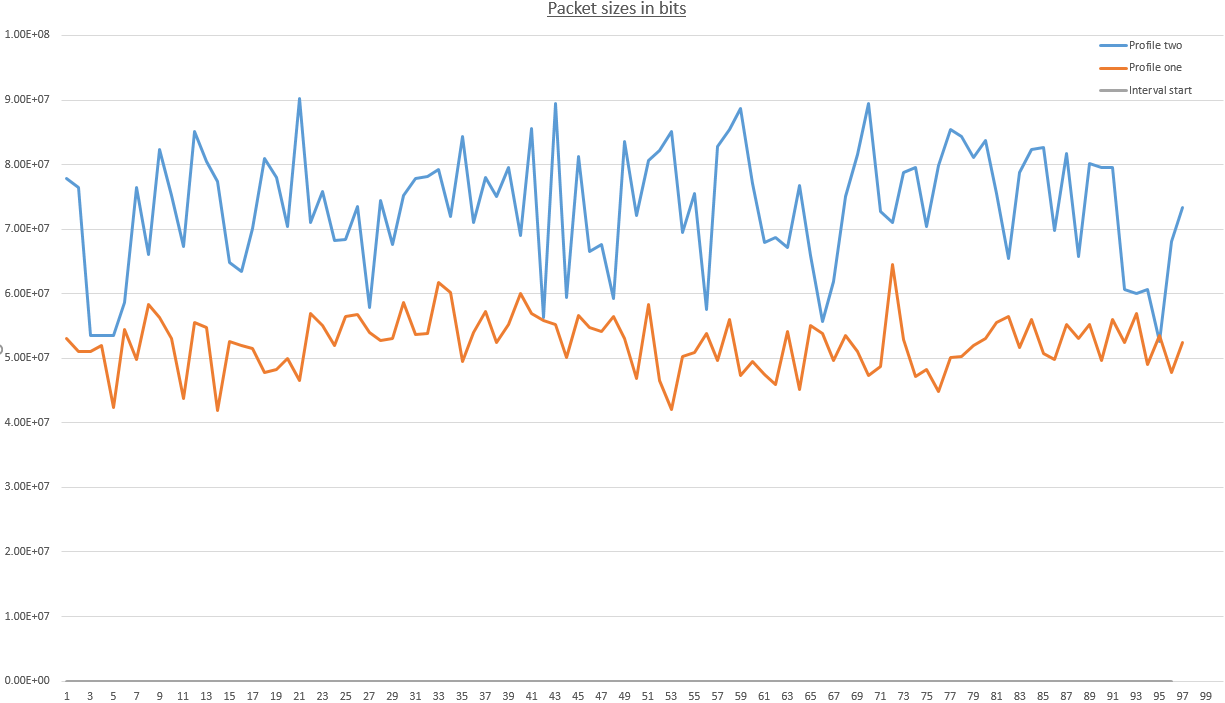
\includegraphics[scale=0.3]{images/wireshark_general.jpg}
    \caption{size of point-clouds streamed, }
    \label{fig:dataPipe}
\end{figure}

\textit{Analysis: What are the challenges?}
\begin{itemize}
    \item Point clouds are very bulky,Figure \ref{fig:dataPipe} shows the size of packets streamed to the master station from camera with 640X480 resolution (Profile one) and profile two shows the size of the packets from two cameras with the same resolution (640x480). as can be seen in the graph the size of the packets is big with average size of  50 and 70 Mega bits respectively.
    \item This huge number of point need a lot's of computational power to process.
    \item because of the size and the lack of efficient compression algorithms the data transmission rate is low.
\end{itemize}


\textbf{Real-time 3D reconstruction with Point-cloud Fusion}

The implemented video feedback from monocular and stereoscopic videos in VR headsets allow operators to look in a fixed direction, but these video interfaces do not respond to any head motion such as moving left/right, forward/backward or up/down. Truly immersive Interface, on the other hand, requires ‘freedom of motion’ in six-degrees-of-freedom (‘6-DoF’), so that operators see the correct views of an environment regardless of where he is (3 DoF) and where he is looking (+3 DoF).

I have integrated a 3D reconstruct algorithm, which reconstructs the FIELD environment in real-time and Showing the 3D reconstruction of the environment to the operator in real-time as the remote robot moves through the field. As a result, the operator could navigate the FIELD environment with much better freedom of motion.

The algorithm is based on the state of the artwork real-time dense visual SLAM algorithm Elastic Fusion [3]. The system is capable of capturing comprehensive dense globally consistent surfel-based maps of an environment and beyond explored using an RGB-D camera in an incremental online fashion, without pose graph optimization or any post-processing steps. This is accomplished by using dense frame-to model camera tracking and windowed surfel-based fusion coupled with frequent model refinement through non-rigid surface deformations.

\begin{figure}[h]
    \centering
    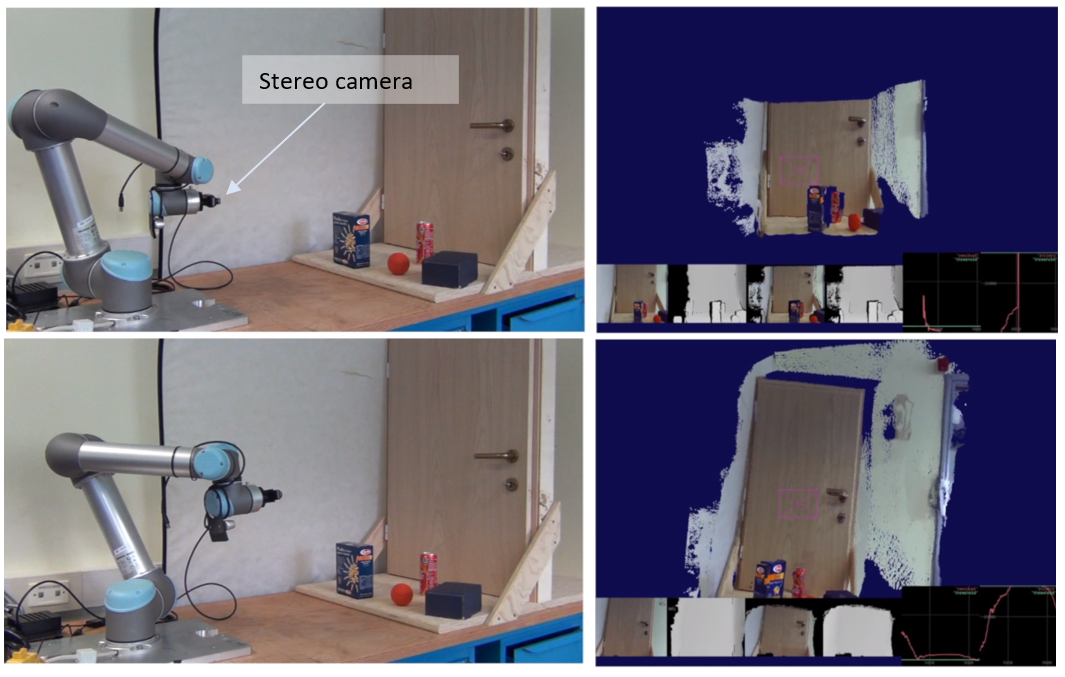
\includegraphics[scale=0.5]{images/Elastic_Fusion.PNG}
    \caption{Real-time 3D reconstruction of static environment for teleoperation.}
    \label{fig:Elastic}
\end{figure}

The algorithm applies local model-to-model surface loop closure optimizations as often as possible to stay close to the mode of the map distribution while utilizing global loop closure to recover from arbitrary drift and maintain global consistency. In the spirit of improving map quality as well as tracking accuracy and robustness, the algorithm furthermore, explore a novel approach to real-time discrete light source detection.

Figure \ref{fig:Elastic} shows 3D reconstructed environment with the corresponding camera and robot position, the stereo camera mounted on the robot end-effector provides the real-time point cloud of the scene and   the algorithm [3] fuses them to generate the full 3D reconstruction of the environment.

\textit{Analysis: What are the challenges ?}
\begin{itemize}
    \item This approach only works for static environment.
    \item Highly resource intensive (the reconstruction continues to grow in time even as it continuously explore a
single static scene).
\end{itemize}

\section{Research Plan}

During the first Ph.D. year, I have focused on researching the state-of-the-art to understand the limitation of 3D immersive interface design for remote teleoperation. In particular, I focused on Augmented reality interfaces and real-time 3D reconstruction. Also for a deeper understanding of the problem, I planned to implement some applications.

The work plans are presented in the Table \ref{table:plan} shown below and it has been distributed to make it consistent with literature review , where the end of literature review and the end of each project considered as a milestone.

\begin{table}[ht] 
\begin{tabular}{ p{4.5cm} p{10cm}}
 \hline
% \multicolumn{4}{|c|}{Country List} \\
% \hline
 \rowcolor{lightgray}  Duration & Research and project \\
\hline

 1 October - 13 December &  Literature review on factors which affect remote tele-operation. \\

\rowcolor{lightgray} 1 October - 31 December &  Implement low latency video streaming. \\

 28 December - 23 March &  Literature review on Augmented Reality interface. \\

\rowcolor{lightgray} 5 February - 23 April: & Implement Augmented Reality Interface. \\

 24 April - 19 July & Literature review on Real-time 3D reconstruction. \\

\rowcolor{lightgray} June 17 &  PhD day poster presentation.\\

 1 June - 31 July & Implement Point-cloud streaming framework.\\
 
 \rowcolor{lightgray} 1 August - 20 September &  Integrate the applications.\\

\end{tabular}
\caption{A list of research and projects for first year}
\label{table:plan}
\end{table}

\subsection*{Future Research Plan}

Following the literature review and the projects have implemented so far, the research will continue to study how operators engage in virtually replicated 3D models of environments and I will try to understand the effect of different artifacts.

An experiment will be designed to include different levels of 3D model representations by changing the fidelity (resolution/density) of the models being displayed and the number of components. alongside a real-time 3D reconstruction algorithm for dynamic environment will be implemented. 

Based on this study, I will design a systematic region selection mechanisms to select relevant and irrelevant information to prioritize computational demand. one of the methods to select region is to use a "Visual attention" mechanisms which is inspired by the human visual system will be used to select important areas of the visual field \textbf{(for alerting)} the operator and to search a target in cluttered scenes \textbf{(searching)}. I will design the models by taking information from the operator, task, sensors and the mission(goal). 

Figure \ref{fig:Attention} shows a systematic diagram of the system model, the attention model will decide the priority of the selected region based on the knowledge from the operator and sensor inputs. a priority will be given to the selected region based on there associated weight. Because of this, the system will have enough computational capability to process each important regions with better quality. moreover, It will help to reduce the size of the data. An overview of the project timeline incorporating the key activities is listed in Table \ref{fig:Plan}.

\begin{figure}[h]
    \centering
    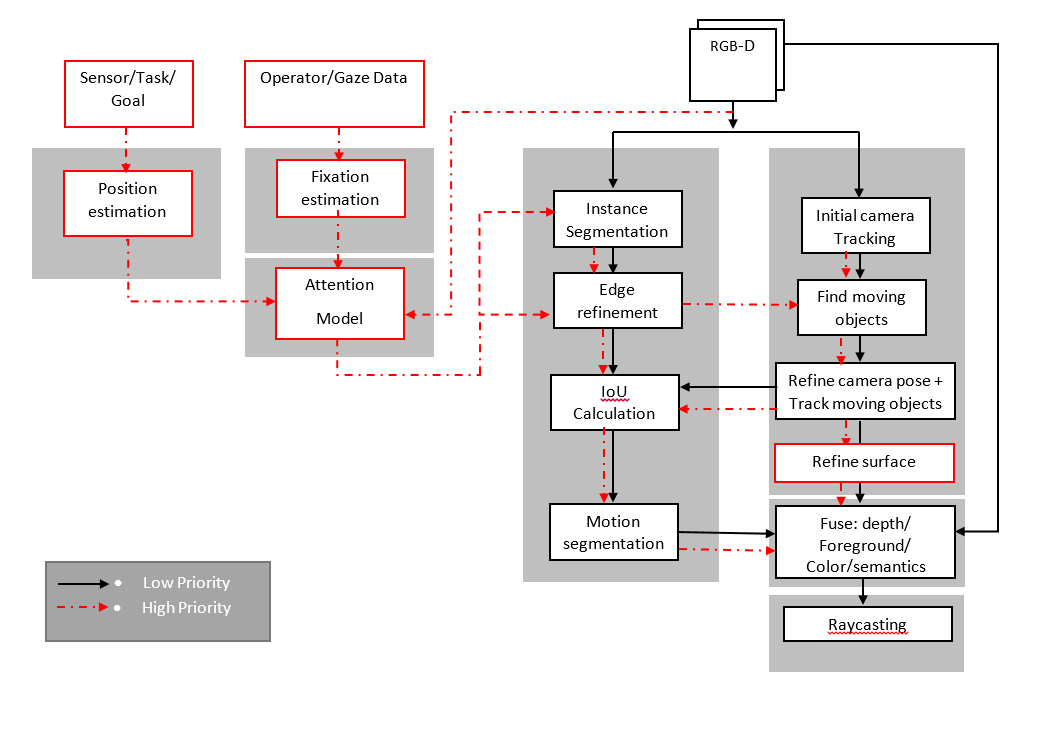
\includegraphics[scale=0.55]{images/Dyn_Reco_Attention.PNG}
    \caption{Real-time 3D reconstruction of dynamic environment using attention models}
    \label{fig:Attention}
\end{figure}

%In the near future, I will continue to develop instance level 3D reconstruction algorithm for dynamic environment. Once these algorithm established,  I will carry on studying How operators navigate and interact with virtually replicated 3D environment to understand and model an attention model shown in Figure \ref{fig:Attention}.

%In the long-term,  I will complete the development of Attention aware dynamic environment 3D reconstruction algorithm. 

\textbf{\textit{Year Two: October 2019 - September 2020}}
\begin{itemize}
    \item Conduct user-study on how users engage in virtually replicated 3D models of environments.
    \item Conduct experiments and collect data.
    \item Write a research paper about the experimented results.
    \item Implement real-time dynamic environment 3D reconstruction algorithm.
    \item Design Attention model based on the results of the study.
    \item Combine the attention model with the Dynamic 3D reconstruction algorithm.
    \item Evaluate the Implemented algorithms for computational efficiency and Quality. 
    \item Refine the total system according to the evaluation results.
    \item Conduct experiments and compare with other approaches.
    \item Write a research paper about the experimented results.
\end{itemize}

\textbf{\textit{Year Three: October 2020 - September 2021}}
\begin{itemize}
    \item Explore if the designed algorithm is suitable for point-cloud compression.
    \item Conduct experiments and compare with other approaches.
    \item Write a research paper about the experimented results
    \item Write thesis & Defend.
\end{itemize} 

\begin{sidewaysfigure}
     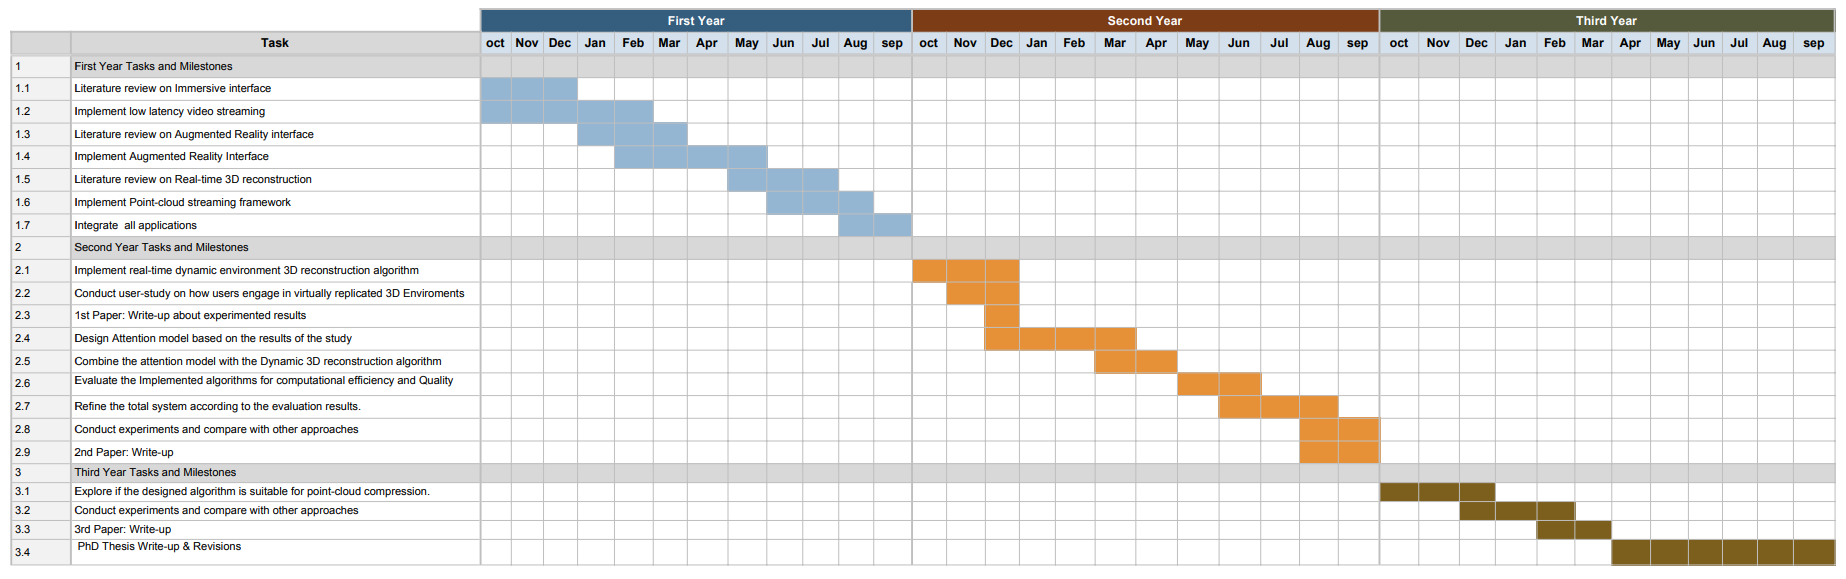
\includegraphics[scale=0.5]{images/GantChart_Table.PNG}
 \caption{Overview of the project plan}
    \label{fig:Plan}
\end{sidewaysfigure} % Introduction

\chapter{Research Aims}

Lorem ipsum dolor sit amet, consectetur adipiscing elit. Vivamus at pulvinar nisi. Phasellus hendrerit, diam placerat interdum iaculis, mauris justo cursus risus, in viverra purus eros at ligula. Ut metus justo, consequat a tristique posuere, laoreet nec nibh. Etiam et scelerisque mauris. Phasellus vel massa magna. Ut non neque id tortor pharetra bibendum vitae sit amet nisi. Duis nec quam quam, sed euismod justo. Pellentesque eu tellus vitae ante tempus malesuada. Nunc accumsan, quam in congue consequat, lectus lectus dapibus erat, id aliquet urna neque at massa. Nulla facilisi. Morbi ullamcorper eleifend posuere. Donec libero leo, faucibus nec bibendum at, mattis et urna. Proin consectetur, nunc ut imperdiet lobortis, magna neque tincidunt lectus, id iaculis nisi justo id nibh. Pellentesque vel sem in erat vulputate faucibus molestie ut lorem.

\section{A Section}

Quisque tristique urna in lorem laoreet at laoreet quam congue. Donec dolor turpis, blandit non imperdiet aliquet, blandit et felis. In lorem nisi, pretium sit amet vestibulum sed, tempus et sem. Proin non ante turpis. Nulla imperdiet fringilla convallis. Vivamus vel bibendum nisl. Pellentesque justo lectus, molestie vel luctus sed, lobortis in libero. Nulla facilisi. Aliquam erat volutpat. Suspendisse vitae nunc nunc. Sed aliquet est suscipit sapien rhoncus non adipiscing nibh consequat. Aliquam metus urna, faucibus eu vulputate non, luctus eu justo.

\subsection{A Subsection}

Donec urna leo, vulputate vitae porta eu, vehicula blandit libero. Phasellus eget massa et leo condimentum mollis. Nullam molestie, justo at pellentesque vulputate, sapien velit ornare diam, nec gravida lacus augue non diam. Integer mattis lacus id libero ultrices sit amet mollis neque molestie. Integer ut leo eget mi volutpat congue. Vivamus sodales, turpis id venenatis placerat, tellus purus adipiscing magna, eu aliquam nibh dolor id nibh. Pellentesque habitant morbi tristique senectus et netus et malesuada fames ac turpis egestas. Sed cursus convallis quam nec vehicula. Sed vulputate neque eget odio fringilla ac sodales urna feugiat.

\section{Another Section}

Phasellus nisi quam, volutpat non ullamcorper eget, congue fringilla leo. Cras et erat et nibh placerat commodo id ornare est. Nulla facilisi. Aenean pulvinar scelerisque eros eget interdum. Nunc pulvinar magna ut felis varius in hendrerit dolor accumsan. Nunc pellentesque magna quis magna bibendum non laoreet erat tincidunt. Nulla facilisi.

Duis eget massa sem, gravida interdum ipsum. Nulla nunc nisl, hendrerit sit amet commodo vel, varius id tellus. Lorem ipsum dolor sit amet, consectetur adipiscing elit. Nunc ac dolor est. Suspendisse ultrices tincidunt metus eget accumsan. Nullam facilisis, justo vitae convallis sollicitudin, eros augue malesuada metus, nec sagittis diam nibh ut sapien. Duis blandit lectus vitae lorem aliquam nec euismod nisi volutpat. Vestibulum ornare dictum tortor, at faucibus justo tempor non. Nulla facilisi. Cras non massa nunc, eget euismod purus. Nunc metus ipsum, euismod a consectetur vel, hendrerit nec nunc. % Background Theory 

\chapter{Background Research}

Lorem ipsum dolor sit amet, consectetur adipiscing elit. Vivamus at pulvinar nisi. Phasellus hendrerit, diam placerat interdum iaculis, mauris justo cursus risus, in viverra purus eros at ligula. Ut metus justo, consequat a tristique posuere, laoreet nec nibh. Etiam et scelerisque mauris. Phasellus vel massa magna. Ut non neque id tortor pharetra bibendum vitae sit amet nisi. Duis nec quam quam, sed euismod justo. Pellentesque eu tellus vitae ante tempus malesuada. Nunc accumsan, quam in congue consequat, lectus lectus dapibus erat, id aliquet urna neque at massa. Nulla facilisi. Morbi ullamcorper eleifend posuere. Donec libero leo, faucibus nec bibendum at, mattis et urna. Proin consectetur, nunc ut imperdiet lobortis, magna neque tincidunt lectus, id iaculis nisi justo id nibh. Pellentesque vel sem in erat vulputate faucibus molestie ut lorem.

\section{A Section}

Quisque tristique urna in lorem laoreet at laoreet quam congue. Donec dolor turpis, blandit non imperdiet aliquet, blandit et felis. In lorem nisi, pretium sit amet vestibulum sed, tempus et sem. Proin non ante turpis. Nulla imperdiet fringilla convallis. Vivamus vel bibendum nisl. Pellentesque justo lectus, molestie vel luctus sed, lobortis in libero. Nulla facilisi. Aliquam erat volutpat. Suspendisse vitae nunc nunc. Sed aliquet est suscipit sapien rhoncus non adipiscing nibh consequat. Aliquam metus urna, faucibus eu vulputate non, luctus eu justo.

\subsection{A Subsection}

Donec urna leo, vulputate vitae porta eu, vehicula blandit libero. Phasellus eget massa et leo condimentum mollis. Nullam molestie, justo at pellentesque vulputate, sapien velit ornare diam, nec gravida lacus augue non diam. Integer mattis lacus id libero ultrices sit amet mollis neque molestie. Integer ut leo eget mi volutpat congue. Vivamus sodales, turpis id venenatis placerat, tellus purus adipiscing magna, eu aliquam nibh dolor id nibh. Pellentesque habitant morbi tristique senectus et netus et malesuada fames ac turpis egestas. Sed cursus convallis quam nec vehicula. Sed vulputate neque eget odio fringilla ac sodales urna feugiat.

\section{Another Section}

Phasellus nisi quam, volutpat non ullamcorper eget, congue fringilla leo. Cras et erat et nibh placerat commodo id ornare est. Nulla facilisi. Aenean pulvinar scelerisque eros eget interdum. Nunc pulvinar magna ut felis varius in hendrerit dolor accumsan. Nunc pellentesque magna quis magna bibendum non laoreet erat tincidunt. Nulla facilisi.

Duis eget massa sem, gravida interdum ipsum. Nulla nunc nisl, hendrerit sit amet commodo vel, varius id tellus. Lorem ipsum dolor sit amet, consectetur adipiscing elit. Nunc ac dolor est. Suspendisse ultrices tincidunt metus eget accumsan. Nullam facilisis, justo vitae convallis sollicitudin, eros augue malesuada metus, nec sagittis diam nibh ut sapien. Duis blandit lectus vitae lorem aliquam nec euismod nisi volutpat. Vestibulum ornare dictum tortor, at faucibus justo tempor non. Nulla facilisi. Cras non massa nunc, eget euismod purus. Nunc metus ipsum, euismod a consectetur vel, hendrerit nec nunc. % Experimental Setup

%
\chapter{Research Plan}

Lorem ipsum dolor sit amet, consectetur adipiscing elit. Vivamus at pulvinar nisi. Phasellus hendrerit, diam placerat interdum iaculis, mauris justo cursus risus, in viverra purus eros at ligula. Ut metus justo, consequat a tristique posuere, laoreet nec nibh. Etiam et scelerisque mauris. Phasellus vel massa magna. Ut non neque id tortor pharetra bibendum vitae sit amet nisi. Duis nec quam quam, sed euismod justo. Pellentesque eu tellus vitae ante tempus malesuada. Nunc accumsan, quam in congue consequat, lectus lectus dapibus erat, id aliquet urna neque at massa. Nulla facilisi. Morbi ullamcorper eleifend posuere. Donec libero leo, faucibus nec bibendum at, mattis et urna. Proin consectetur, nunc ut imperdiet lobortis, magna neque tincidunt lectus, id iaculis nisi justo id nibh. Pellentesque vel sem in erat vulputate faucibus molestie ut lorem.

\section{A Section}

Quisque tristique urna in lorem laoreet at laoreet quam congue. Donec dolor turpis, blandit non imperdiet aliquet, blandit et felis. In lorem nisi, pretium sit amet vestibulum sed, tempus et sem. Proin non ante turpis. Nulla imperdiet fringilla convallis. Vivamus vel bibendum nisl. Pellentesque justo lectus, molestie vel luctus sed, lobortis in libero. Nulla facilisi. Aliquam erat volutpat. Suspendisse vitae nunc nunc. Sed aliquet est suscipit sapien rhoncus non adipiscing nibh consequat. Aliquam metus urna, faucibus eu vulputate non, luctus eu justo.

\subsection{A Subsection}

Donec urna leo, vulputate vitae porta eu, vehicula blandit libero. Phasellus eget massa et leo condimentum mollis. Nullam molestie, justo at pellentesque vulputate, sapien velit ornare diam, nec gravida lacus augue non diam. Integer mattis lacus id libero ultrices sit amet mollis neque molestie. Integer ut leo eget mi volutpat congue. Vivamus sodales, turpis id venenatis placerat, tellus purus adipiscing magna, eu aliquam nibh dolor id nibh. Pellentesque habitant morbi tristique senectus et netus et malesuada fames ac turpis egestas. Sed cursus convallis quam nec vehicula. Sed vulputate neque eget odio fringilla ac sodales urna feugiat.

\section{Another Section}

Phasellus nisi quam, volutpat non ullamcorper eget, congue fringilla leo. Cras et erat et nibh placerat commodo id ornare est. Nulla facilisi. Aenean pulvinar scelerisque eros eget interdum. Nunc pulvinar magna ut felis varius in hendrerit dolor accumsan. Nunc pellentesque magna quis magna bibendum non laoreet erat tincidunt. Nulla facilisi.

Duis eget massa sem, gravida interdum ipsum. Nulla nunc nisl, hendrerit sit amet commodo vel, varius id tellus. Lorem ipsum dolor sit amet, consectetur adipiscing elit. Nunc ac dolor est. Suspendisse ultrices tincidunt metus eget accumsan. Nullam facilisis, justo vitae convallis sollicitudin, eros augue malesuada metus, nec sagittis diam nibh ut sapien. Duis blandit lectus vitae lorem aliquam nec euismod nisi volutpat. Vestibulum ornare dictum tortor, at faucibus justo tempor non. Nulla facilisi. Cras non massa nunc, eget euismod purus. Nunc metus ipsum, euismod a consectetur vel, hendrerit nec nunc. % Experiment 1

%\input{Chapters/Chapter5} % Experiment 2

%\input{Chapters/Chapter6} % Results and Discussion

%\input{Chapters/Chapter7} % Conclusion

%% ----------------------------------------------------------------
% Now begin the Appendices, including them as separate files

\addtocontents{toc}{\vspace{2em}} % Add a gap in the Contents, for aesthetics

\appendix % Cue to tell LaTeX that the following 'chapters' are Appendices

\chapter{An Appendix}

Lorem ipsum dolor sit amet, consectetur adipiscing elit. Vivamus at pulvinar nisi. Phasellus hendrerit, diam placerat interdum iaculis, mauris justo cursus risus, in viverra purus eros at ligula. Ut metus justo, consequat a tristique posuere, laoreet nec nibh. Etiam et scelerisque mauris. Phasellus vel massa magna. Ut non neque id tortor pharetra bibendum vitae sit amet nisi. Duis nec quam quam, sed euismod justo. Pellentesque eu tellus vitae ante tempus malesuada. Nunc accumsan, quam in congue consequat, lectus lectus dapibus erat, id aliquet urna neque at massa. Nulla facilisi. Morbi ullamcorper eleifend posuere. Donec libero leo, faucibus nec bibendum at, mattis et urna. Proin consectetur, nunc ut imperdiet lobortis, magna neque tincidunt lectus, id iaculis nisi justo id nibh. Pellentesque vel sem in erat vulputate faucibus molestie ut lorem.

Quisque tristique urna in lorem laoreet at laoreet quam congue. Donec dolor turpis, blandit non imperdiet aliquet, blandit et felis. In lorem nisi, pretium sit amet vestibulum sed, tempus et sem. Proin non ante turpis. Nulla imperdiet fringilla convallis. Vivamus vel bibendum nisl. Pellentesque justo lectus, molestie vel luctus sed, lobortis in libero. Nulla facilisi. Aliquam erat volutpat. Suspendisse vitae nunc nunc. Sed aliquet est suscipit sapien rhoncus non adipiscing nibh consequat. Aliquam metus urna, faucibus eu vulputate non, luctus eu justo.

Donec urna leo, vulputate vitae porta eu, vehicula blandit libero. Phasellus eget massa et leo condimentum mollis. Nullam molestie, justo at pellentesque vulputate, sapien velit ornare diam, nec gravida lacus augue non diam. Integer mattis lacus id libero ultrices sit amet mollis neque molestie. Integer ut leo eget mi volutpat congue. Vivamus sodales, turpis id venenatis placerat, tellus purus adipiscing magna, eu aliquam nibh dolor id nibh. Pellentesque habitant morbi tristique senectus et netus et malesuada fames ac turpis egestas. Sed cursus convallis quam nec vehicula. Sed vulputate neque eget odio fringilla ac sodales urna feugiat.

Phasellus nisi quam, volutpat non ullamcorper eget, congue fringilla leo. Cras et erat et nibh placerat commodo id ornare est. Nulla facilisi. Aenean pulvinar scelerisque eros eget interdum. Nunc pulvinar magna ut felis varius in hendrerit dolor accumsan. Nunc pellentesque magna quis magna bibendum non laoreet erat tincidunt. Nulla facilisi.

Duis eget massa sem, gravida interdum ipsum. Nulla nunc nisl, hendrerit sit amet commodo vel, varius id tellus. Lorem ipsum dolor sit amet, consectetur adipiscing elit. Nunc ac dolor est. Suspendisse ultrices tincidunt metus eget accumsan. Nullam facilisis, justo vitae convallis sollicitudin, eros augue malesuada metus, nec sagittis diam nibh ut sapien. Duis blandit lectus vitae lorem aliquam nec euismod nisi volutpat. Vestibulum ornare dictum tortor, at faucibus justo tempor non. Nulla facilisi. Cras non massa nunc, eget euismod purus. Nunc metus ipsum, euismod a consectetur vel, hendrerit nec nunc.	% Appendix Title

%\input{Appendices/AppendixB} % Appendix Title

%\input{Appendices/AppendixC} % Appendix Title

\addtocontents{toc}{\vspace{2em}}  % Add a gap in the Contents, for aesthetics
\backmatter

%% ----------------------------------------------------------------
\label{Bibliography}
\lhead{\emph{Bibliography}}  % Change the left side page header to "Bibliography"
\bibliographystyle{unsrtnat}  % Use the "unsrtnat" BibTeX style for formatting the Bibliography
\bibliography{Bibliography}  % The references (bibliography) information are stored in the file named "Bibliography.bib"

\end{document}  % The End
%% ----------------------------------------------------------------